\PassOptionsToPackage{unicode=true}{hyperref} % options for packages loaded elsewhere
\PassOptionsToPackage{hyphens}{url}
%
\documentclass[12pt,ignorenonframetext,]{beamer}
\usepackage{pgfpages}
\setbeamertemplate{caption}[numbered]
\setbeamertemplate{caption label separator}{: }
\setbeamercolor{caption name}{fg=normal text.fg}
\beamertemplatenavigationsymbolsempty
% Prevent slide breaks in the middle of a paragraph:
\widowpenalties 1 10000
\raggedbottom
\setbeamertemplate{part page}{
\centering
\begin{beamercolorbox}[sep=16pt,center]{part title}
  \usebeamerfont{part title}\insertpart\par
\end{beamercolorbox}
}
\setbeamertemplate{section page}{
\centering
\begin{beamercolorbox}[sep=12pt,center]{part title}
  \usebeamerfont{section title}\insertsection\par
\end{beamercolorbox}
}
\setbeamertemplate{subsection page}{
\centering
\begin{beamercolorbox}[sep=8pt,center]{part title}
  \usebeamerfont{subsection title}\insertsubsection\par
\end{beamercolorbox}
}
\AtBeginPart{
  \frame{\partpage}
}
\AtBeginSection{
  \ifbibliography
  \else
    \frame{\sectionpage}
  \fi
}
\AtBeginSubsection{
  \frame{\subsectionpage}
}
\usepackage{lmodern}
\usepackage{amssymb,amsmath}
\usepackage{ifxetex,ifluatex}
\usepackage{fixltx2e} % provides \textsubscript
\ifnum 0\ifxetex 1\fi\ifluatex 1\fi=0 % if pdftex
  \usepackage[T1]{fontenc}
  \usepackage[utf8]{inputenc}
  \usepackage{textcomp} % provides euro and other symbols
\else % if luatex or xelatex
  \usepackage{unicode-math}
  \defaultfontfeatures{Ligatures=TeX,Scale=MatchLowercase}
\fi
\usetheme[]{Frankfurt}
\usecolortheme{lily}
% use upquote if available, for straight quotes in verbatim environments
\IfFileExists{upquote.sty}{\usepackage{upquote}}{}
% use microtype if available
\IfFileExists{microtype.sty}{%
\usepackage[]{microtype}
\UseMicrotypeSet[protrusion]{basicmath} % disable protrusion for tt fonts
}{}
\IfFileExists{parskip.sty}{%
\usepackage{parskip}
}{% else
\setlength{\parindent}{0pt}
\setlength{\parskip}{6pt plus 2pt minus 1pt}
}
\usepackage{hyperref}
\hypersetup{
            pdftitle={Strategic Decision Making in the 3D Printing Industry},
            pdfauthor={Pedro Nascimento de Lima,; Maria I. W. M. Morandi,; Daniel Pacheco Lacerda},
            pdfborder={0 0 0},
            breaklinks=true}
\urlstyle{same}  % don't use monospace font for urls
\newif\ifbibliography
\setlength{\emergencystretch}{3em}  % prevent overfull lines
\providecommand{\tightlist}{%
  \setlength{\itemsep}{0pt}\setlength{\parskip}{0pt}}
\setcounter{secnumdepth}{0}

% set default figure placement to htbp
\makeatletter
\def\fps@figure{htbp}
\makeatother


\def\begincols{\begin{columns}}
\def\begincol{\begin{column}}
\def\endcol{\end{column}}
\def\endcols{\end{columns}}

\AtBeginSubsection{}
\AtBeginSection{}

\setbeamertemplate{footline}[text line]{%
  \parbox{\linewidth}{\vspace*{-8pt}2018 DMDU Meeting\hfill\insertshortauthor\hfill\insertpagenumber}}

\setbeamertemplate{navigation symbols}{}

\title{Strategic Decision Making in the 3D Printing Industry}
\providecommand{\subtitle}[1]{}
\subtitle{A Robust Decision Making (RDM) analysis}
\author{Pedro Nascimento de Lima, \and Maria I. W. M. Morandi, \and Daniel Pacheco Lacerda}
\providecommand{\institute}[1]{}
\institute{GMAP Research Group, UNISINOS University, RS, Brazil \and 2018 DMDU Annual Meeting, California, US}
\date{November 14, 2018}

\begin{document}
\frame{\titlepage}

\hypertarget{introduction}{%
\section{Introduction}\label{introduction}}

\begin{frame}{The 3D Printing Industry}
\protect\hypertarget{the-3d-printing-industry}{}

3D printing, the manufacturing of parts by adding layers of material, is
gaining importance not only for prototyping but also for finished parts
production.

Additive Manufacturing (AM) holds the potential to impact production
systems by:

\begin{itemize}
\tightlist
\item
  Streamlining supply chains;
\item
  Enabling economic manufacturing of customized parts;
\item
  Allowing the production of more efficient technical parts with highly
  complex geometry.
\end{itemize}

\end{frame}

\begin{frame}{Conventional vs 3D Printed Part}
\protect\hypertarget{conventional-vs-3d-printed-part}{}

\centerline{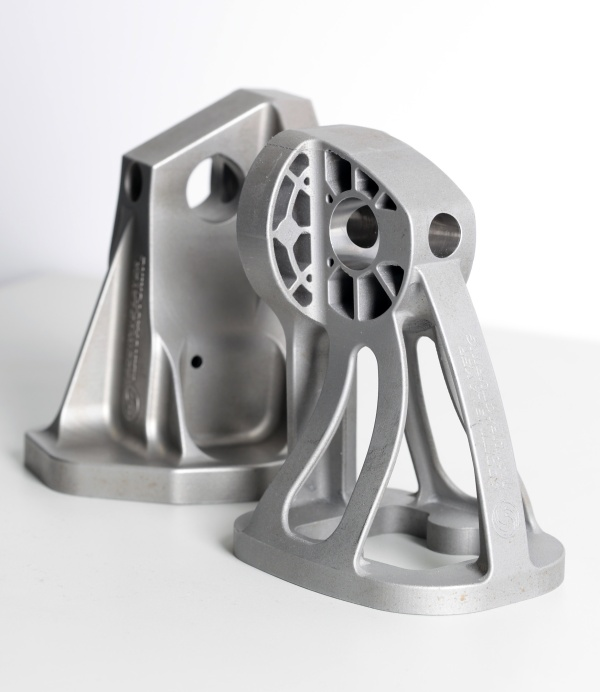
\includegraphics[height=2.5in]{images/conventional-vs-3d.jpg}}

Image Source:
\href{https://www.metal-am.com/introduction-to-metal-additive-manufacturing-and-3d-printing/}{metal-am.com}

\end{frame}

\begin{frame}{Key driving Factors in AM Industry}
\protect\hypertarget{key-driving-factors-in-am-industry}{}

These are a few of the key deeply uncertain factors Challenging AM
Systems Manufacturer's Strategy:

\begin{itemize}
\item
  \textbf{Pace of R \& D and Tech. Improvement}: will our competitors
  develop the next breakthrough in AM?
\item
  \textbf{Patent Dynamics and Expiration}: Can we leverage the benefits
  of our technology before the patent expires? (e.g.: FDM in 2009).
\item
  \textbf{Open Source Players}: Will other major players engage in open
  source technologies or platforms? (e.g.: Prusa).
\item
  \textbf{Aggressive Competition and new entrants}: To what extent can
  we deter new players from aggressively entering the field?
\end{itemize}

\end{frame}

\hypertarget{xlrm}{%
\section{XLRM}\label{xlrm}}

\begin{frame}{New Product Diffusion Models}
\protect\hypertarget{new-product-diffusion-models}{}

There is a broad range of models portraying new product diffusion and
technological substitutions, beyond the basic Bass Diffusion Model (Bass
1969):

\begin{itemize}
\tightlist
\item
  \textbf{New Product Launch Strategy} and Timing Between Successive
  Product Generations (Mahajan and Muller 1996);
\item
  \textbf{Social Factors} (e.g.~Reference Users and Opinion Leaders - GE
  in the case of AM) (Dattée and Birdseye Weil 2007);
\item
  \textbf{Competition} Among Players and Substitution Between Product
  Generations (Maier 1998);
\item
  \textbf{Market Uncertainty} (Cui, Zhao, and Ravichandran 2011);
\item
  \textbf{Competition, Learning Curves, diffusion dynamics, Pricing and
  Capacity Strategies} (Sterman et al. 2007).
\end{itemize}

\end{frame}

\begin{frame}{X - Uncertainties}
\protect\hypertarget{x---uncertainties}{}

This study analyzed \textbf{parametric uncertainty} present in the
professional AM market, represented by 35 model parameters, including:

\begin{itemize}
\tightlist
\item
  \textbf{Diffusion Dynamics parameters}:how fast and to what extent the
  industrial-grade 3D printing market might grow;
\item
  \textbf{Opponent's Strategies}: The strategy of the opponents
  manufacturers are also defined as uncertain;
\item
  \textbf{Market Share}: To what extent the market will prioritize 3D
  printer performance rather than its cost.
\end{itemize}

\end{frame}

\begin{frame}{L - Levers}
\protect\hypertarget{l---levers}{}

The AM Systems Manufacturer is allowed to use four levers:

\begin{enumerate}
\tightlist
\item
  \textbf{Pricing and Capacity Strategy}: Aggressive vs Conservative;
\item
  \textbf{Target Market Share}: 20\%, 30\% or 40\%;
\item
  \textbf{R \& D Budget}: 5\%, 10\% or 15\%;
\item
  \textbf{\% of Open Source R \& D}: 0\%, 50\%, 90\%.
\end{enumerate}

\end{frame}

\begin{frame}{Relationships - Sterman et al. (2007) expanded model}
\protect\hypertarget{relationships---sterman-et-al.-2007-expanded-model}{}

\centerline{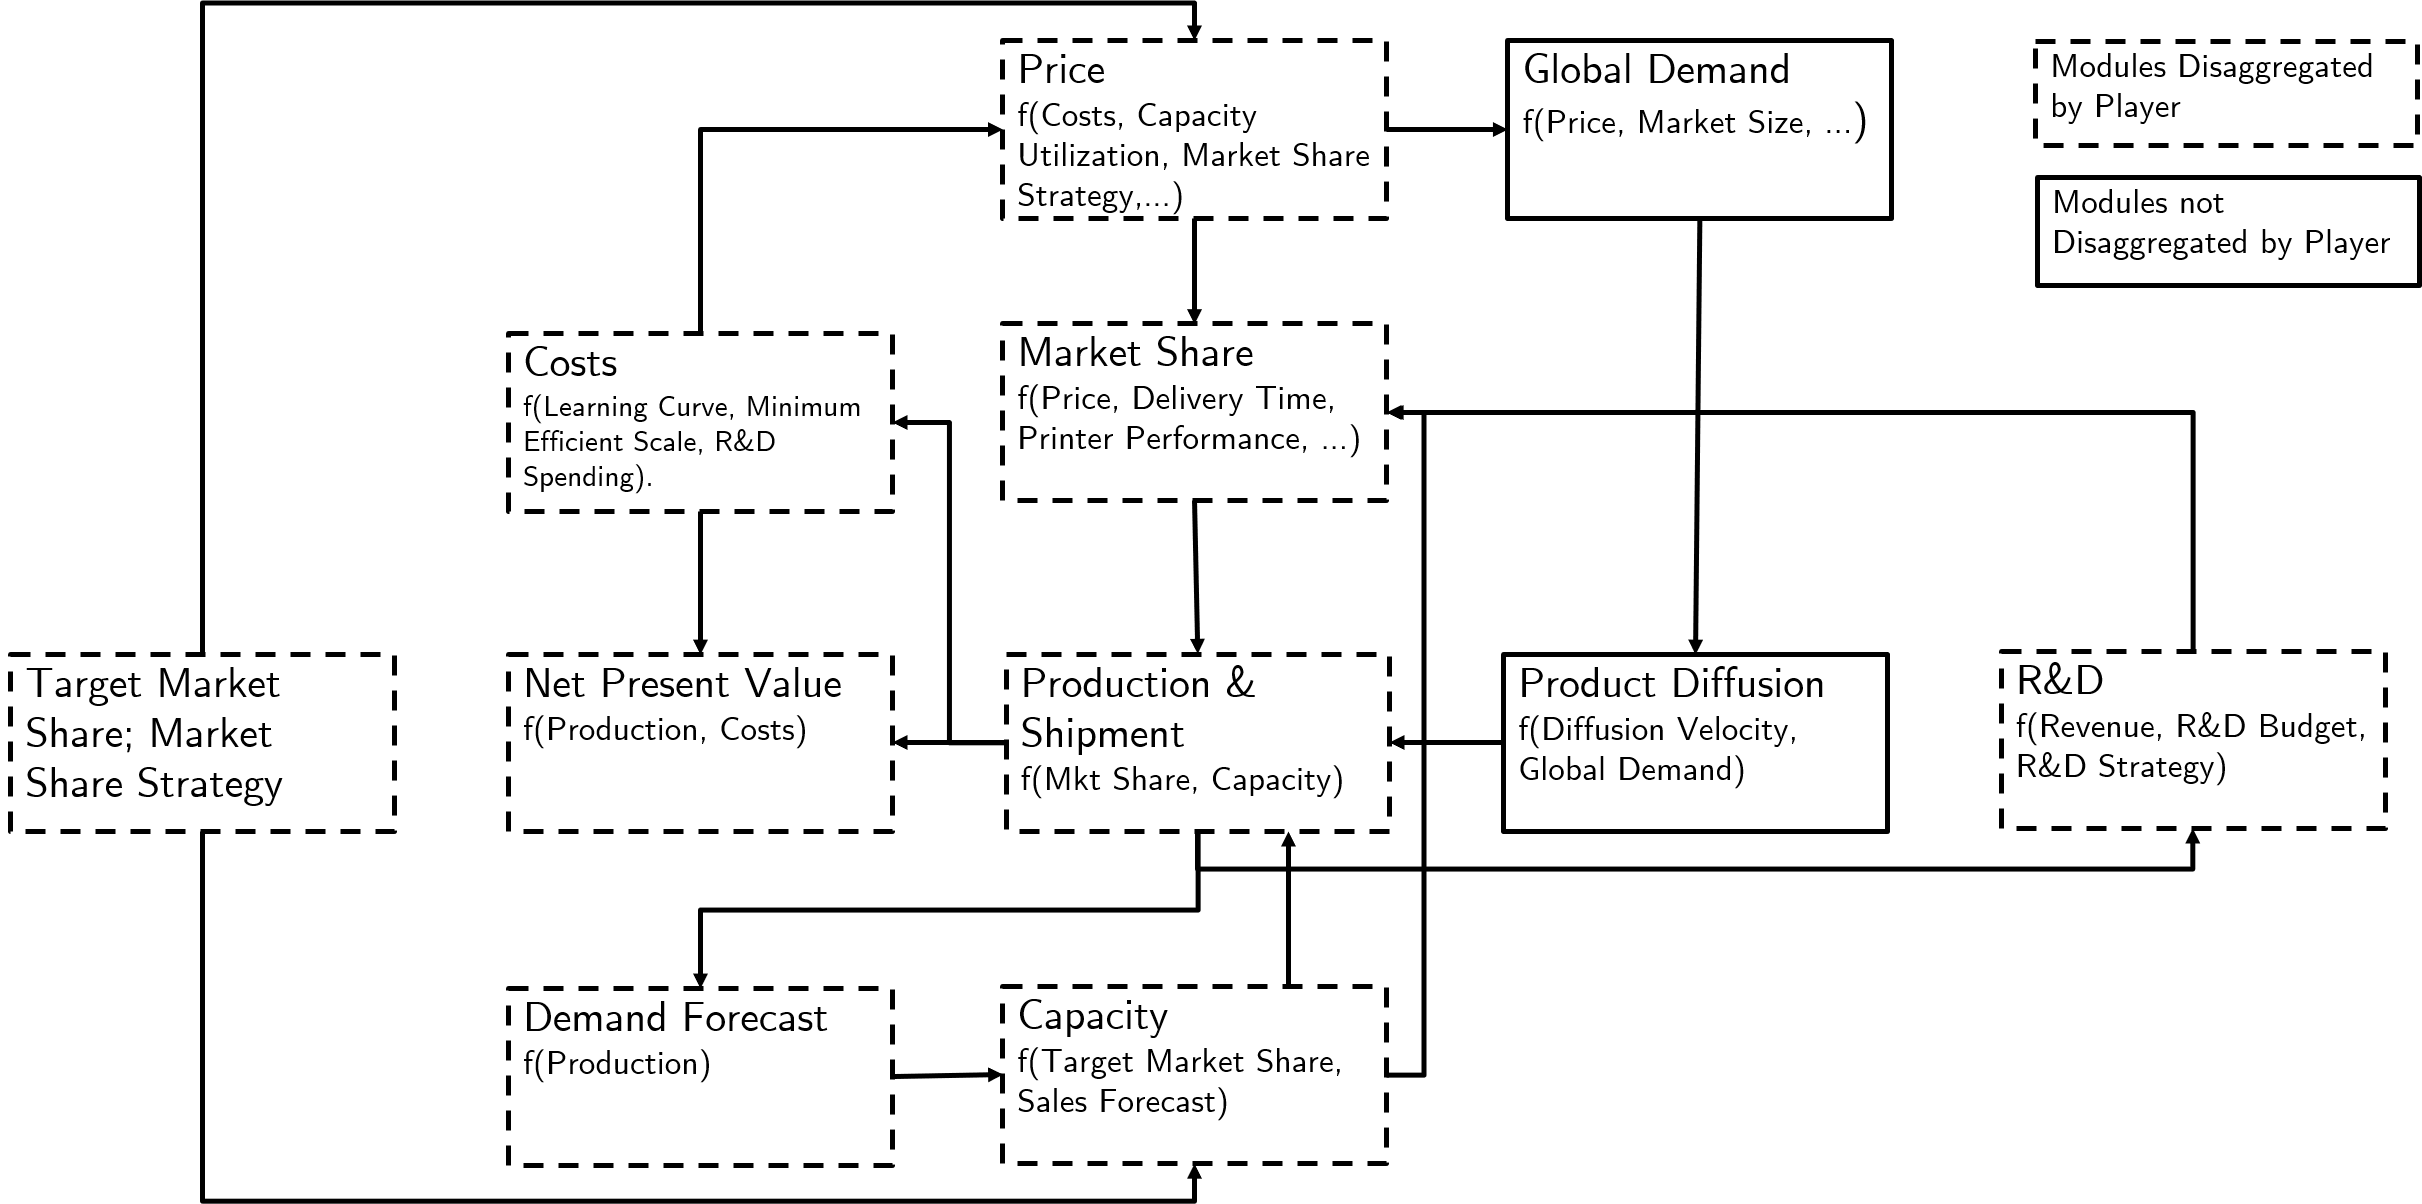
\includegraphics[height=2.5in]{images/model-boundaries.png}}

\end{frame}

\begin{frame}{Relationships - A glimpse* into the model}
\protect\hypertarget{relationships---a-glimpse-into-the-model}{}

\begin{itemize}
\tightlist
\item
  Product Diffusion:
\end{itemize}

\[ A_t = A_{t_0} + \int_{t_0}^{t}  MAX\left(0,N \left(\alpha + \beta \frac{A}{POP}\right)\right); A_{t_0} = \theta A^*\]

\begin{itemize}
\tightlist
\item
  Patent Dynamics (added to the model):
\end{itemize}

\[dT^o/dt = \sum_{i}{[\kappa_i * (1-\psi) * T_i^r / \upsilon^a]}   - T^o/ \upsilon^e \]

*Link to Full documentation, and parameters ranges provided on the final
slide.

\end{frame}

\begin{frame}{Metrics}
\protect\hypertarget{metrics}{}

We use the \textbf{Absolute Regret} of the Player's 1 Net Present Value
as the metric to compare different alternatives.

\end{frame}

\hypertarget{case-generation}{%
\section{Case Generation}\label{case-generation}}

\begin{frame}{Scenario Ensemble}
\protect\hypertarget{scenario-ensemble}{}

\begin{itemize}
\tightlist
\item
  \textbf{Experimental Design}: 54 strategies were obtained through a
  full-factorial design of the levers and their levels.
\item
  \textbf{Results Database:} The simulation results database contains
  10.800 runs (54 strategies X 200 scenarios obtained from LHS of the 35
  uncertain parameters).
\item
  \textbf{Time-frame:} 10 years.
\end{itemize}

\end{frame}

\begin{frame}{Why 3D Printing?}
\protect\hypertarget{why-3d-printing}{}

3D Printing is an emergint technology, but decision makers face
uncertainty:

\begincols
  \begincol{.48\textwidth}

\textbf{Positive Evidence}:

\begin{itemize}
\item
  3D printing Industry has seen two digits growth consistently in the
  last few years;
\item
  3D printing is already reshaping supply chains across industries
  (e.g.: prothesis, aerospace, etc.).

  \endcol
  \begincol{.48\textwidth}
\end{itemize}

\textbf{Negative Evidence}:

\begin{itemize}
\item
  Major players have been observing declining profitability (e.g.:
  Stratasys, 3D Systems);
\item
  Estimates of 3D printing growth diverge.

  \endcol
  \endcols
\end{itemize}

\end{frame}

\begin{frame}{Candidate Strategy NPV across scenarios}
\protect\hypertarget{candidate-strategy-npv-across-scenarios}{}

\centerline{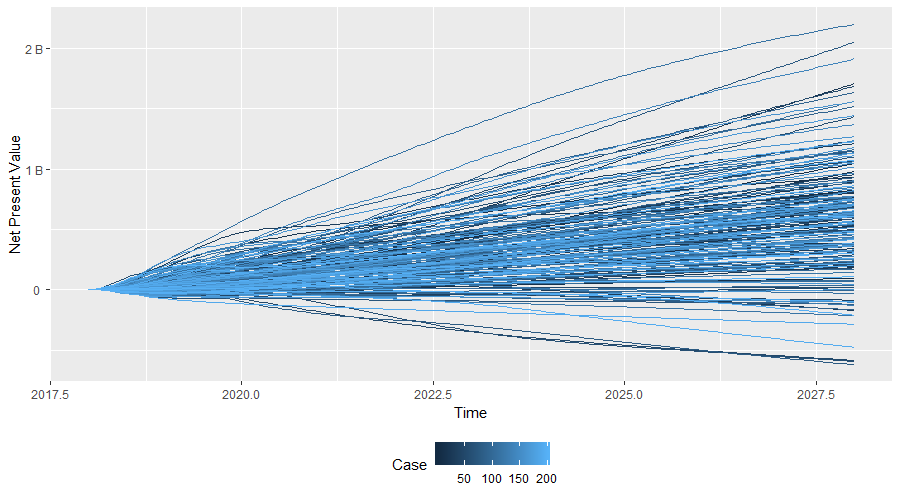
\includegraphics[height=2.5in]{images/npv.png}}

\end{frame}

\begin{frame}{Global Demand across scenarios}
\protect\hypertarget{global-demand-across-scenarios}{}

\centerline{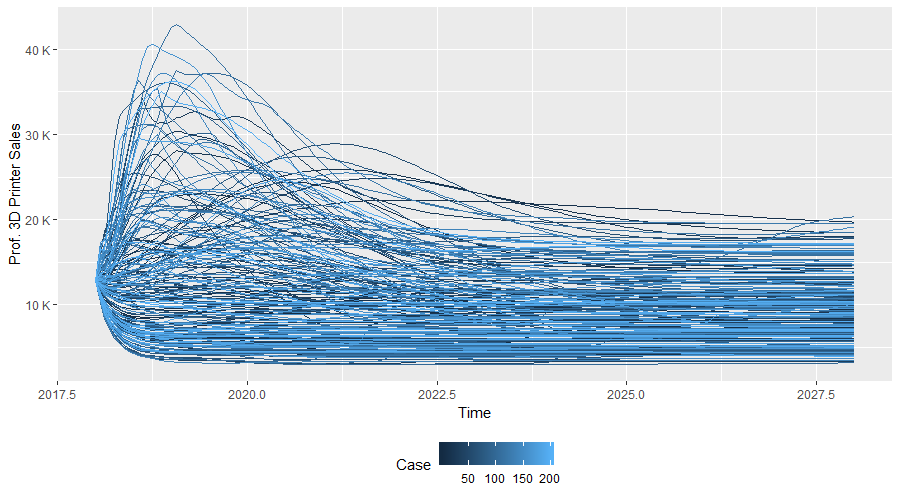
\includegraphics[height=2.5in]{images/sales.png}}

\end{frame}

\begin{frame}{4 Players Net Present Value in a given scenario}
\protect\hypertarget{players-net-present-value-in-a-given-scenario}{}

\centerline{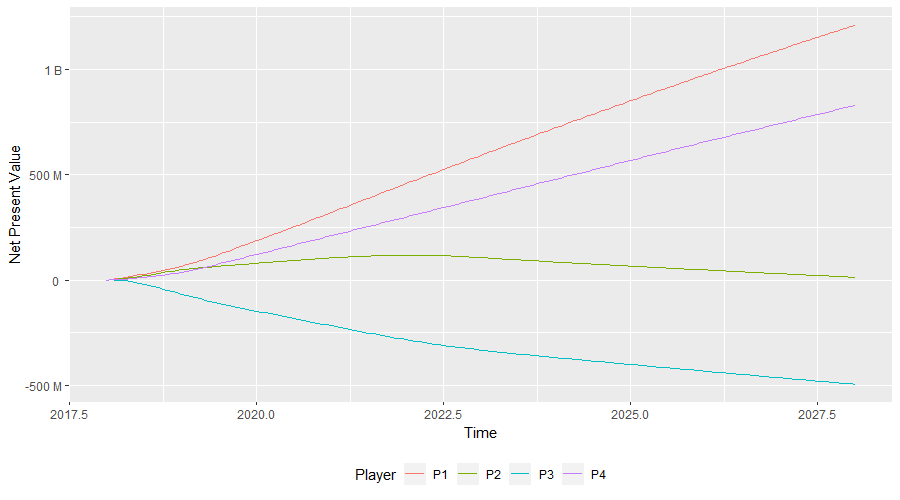
\includegraphics[height=2.5in]{images/npv-players.png}}

\end{frame}

\begin{frame}{Net Present Value across strategies and Scenarios}
\protect\hypertarget{net-present-value-across-strategies-and-scenarios}{}

\centerline{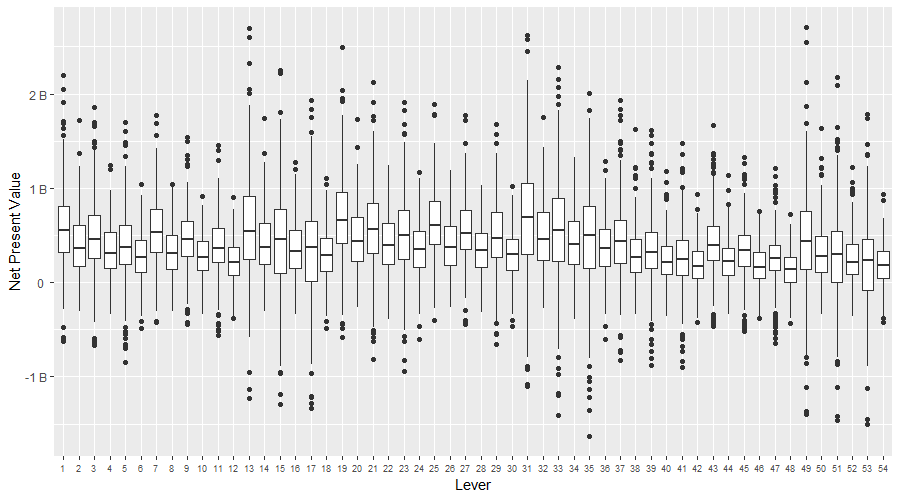
\includegraphics[height=2.5in]{images/npv-whisker.png}}

\end{frame}

\begin{frame}{Regret across strategies and Scenarios}
\protect\hypertarget{regret-across-strategies-and-scenarios}{}

\centerline{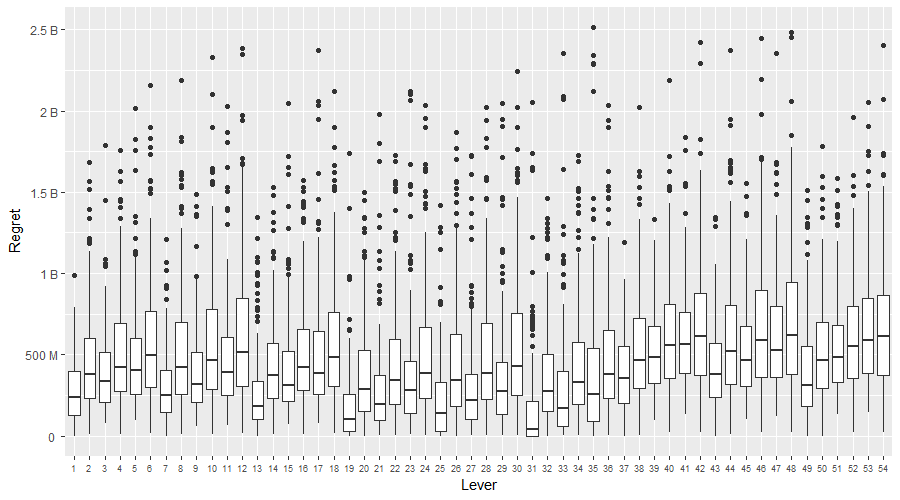
\includegraphics[height=2.5in]{images/regret-whisker.png}}

\end{frame}

\begin{frame}{Selected Candidate Strategy}
\protect\hypertarget{selected-candidate-strategy}{}

\begin{itemize}
\tightlist
\item
  \textbf{Aggressive, Closed Source} Strategies dominated their
  counterparts;
\item
  The strategy with the \textbf{least 75 percentile Regret} was selected
  for vulnerability analysis.
\item
  Under this strategy (31), the player chooses to \textbf{price
  aggressively} with a \textbf{high target market share} (40 \%),
  \textbf{invest less in R \& D} (5\%) with a \textbf{closed source}
  strategy.
\end{itemize}

\end{frame}

\hypertarget{scenario-discovery}{%
\section{Scenario Discovery}\label{scenario-discovery}}

\begin{frame}{Vulnerability Analysis with Random Forests}
\protect\hypertarget{vulnerability-analysis-with-random-forests}{}

\begin{itemize}
\item
  We trained a \textbf{Random Forest}, and employed the \textbf{Boruta
  Algorithm} to identify the most influential uncertainties that define
  the circumstances under which strategy 32 might fail ( Regret
  \textgreater{} 211.9 K USD);
\item
  We use the \textbf{feature importance ranking} from the random forest
  to determine which uncertain parameters are more important to define
  the strategy's failure\ldots{}
\end{itemize}

\end{frame}

\begin{frame}{Visualizing Vulnerabilities with PDPs}
\protect\hypertarget{visualizing-vulnerabilities-with-pdps}{}

\centerline{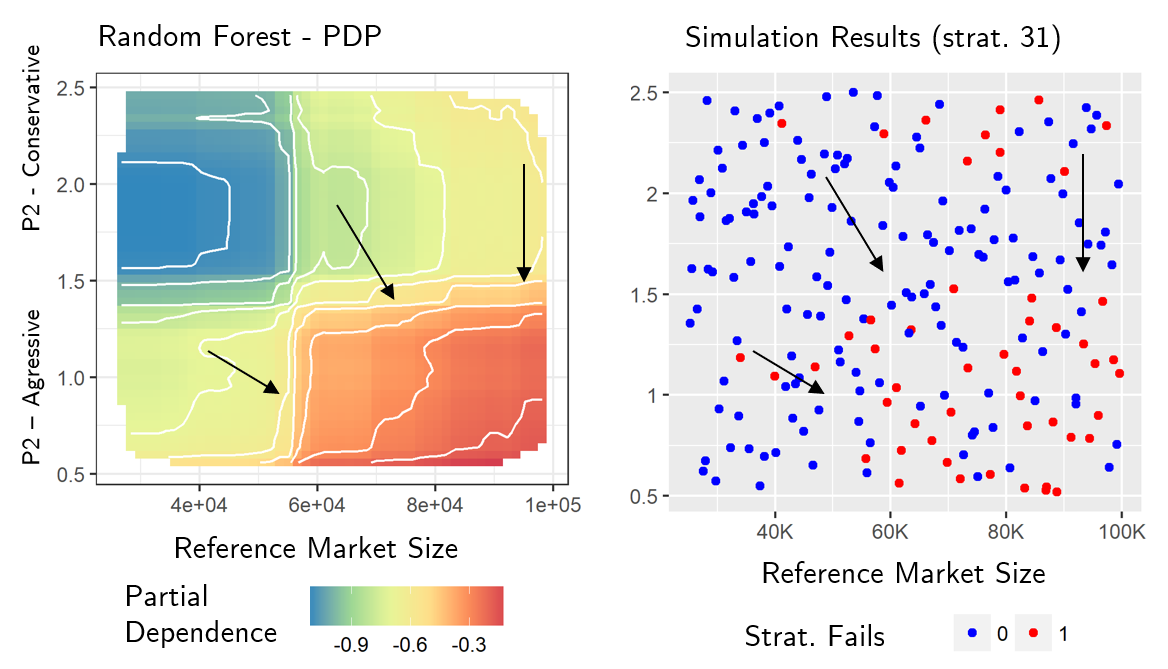
\includegraphics[height=2.5in]{images/pdp-plot.png}}

\end{frame}

\begin{frame}{PRIM}
\protect\hypertarget{prim}{}

PRIM also found a \textbf{high-regret region} where the \textbf{strategy
failed on 82,1 \%} of the futures simulated.

\centerline{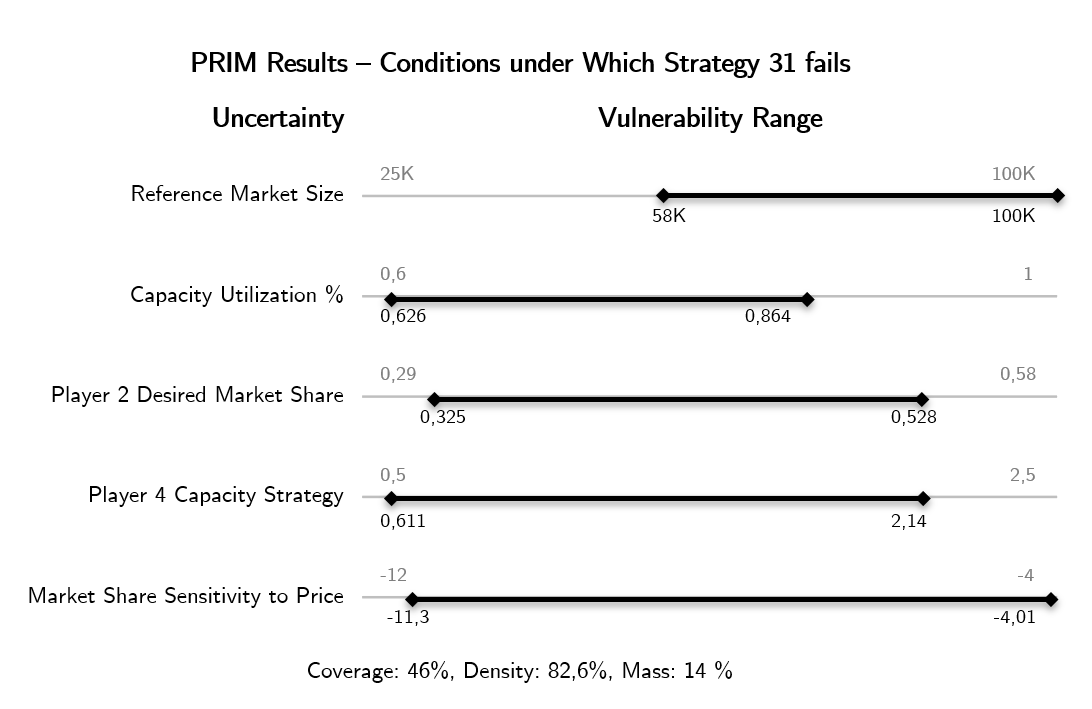
\includegraphics[height=2in]{images/prim-results.png}}

\end{frame}

\hypertarget{trade-off-analysis}{%
\section{Trade-off Analysis}\label{trade-off-analysis}}

\begin{frame}{Trade-off Frontier}
\protect\hypertarget{trade-off-frontier}{}

Trade-off analysis lends \textbf{no support for Open R \& D or
Conservative Strategies}, as the trade-off frontier is dominated by
closed-source, less-aggressive strategies:

\centerline{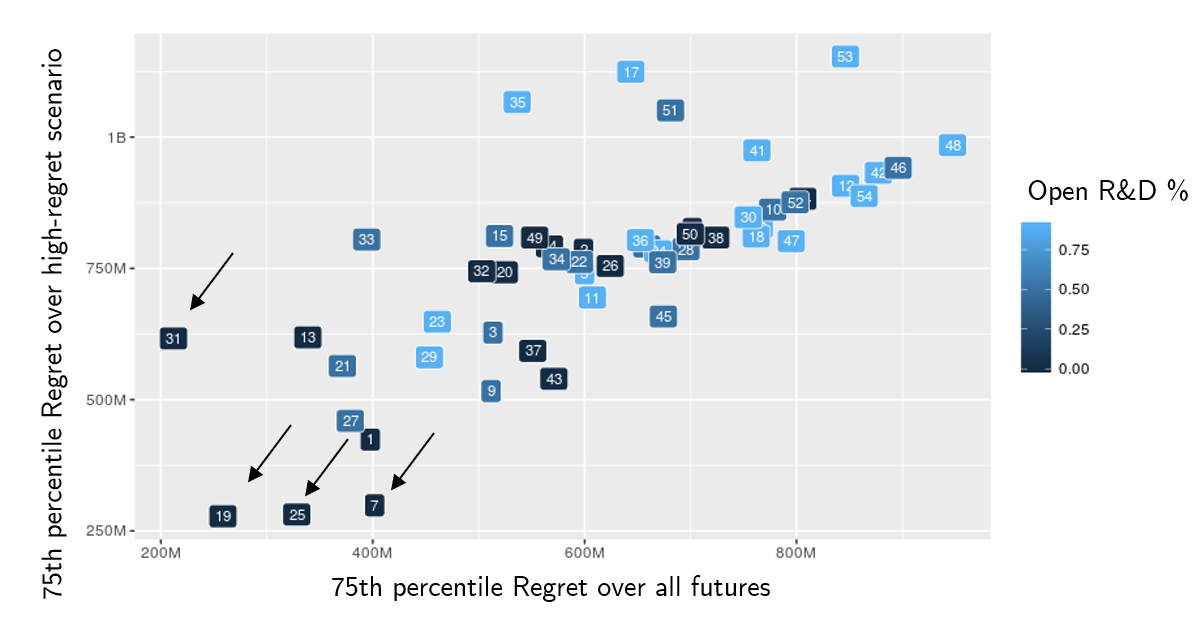
\includegraphics[height=2in]{images/tradeoff-frontier.png}}

\end{frame}

\begin{frame}{Trade-off Curves}
\protect\hypertarget{trade-off-curves}{}

Strategies 25 and 19 still use an aggressive heuristic but \textbf{have
less ambitious target market share}:

\centerline{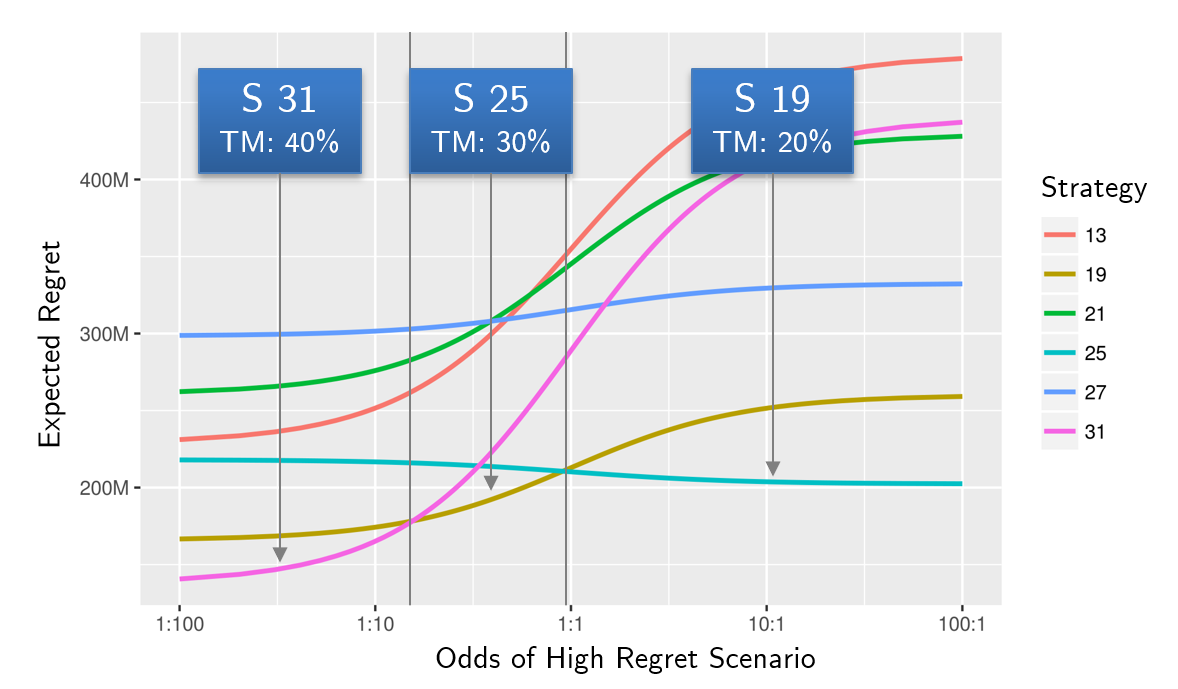
\includegraphics[height=2in]{images/tradeoff-analysis.png}}

\end{frame}

\hypertarget{conclusion}{%
\section{Conclusion}\label{conclusion}}

\begin{frame}{Final Remarks}
\protect\hypertarget{final-remarks}{}

This analysis provides an exploration of model-based Business Strategic
Decision aiding under the DMDU framework.

Future work might either relax some of the structural assumptions of the
model employed on this analysis or turn to new deeply uncertain business
problems.

\end{frame}

\begin{frame}{Questions?}
\protect\hypertarget{questions}{}

\textbf{Questions?}

\end{frame}

\begin{frame}{Further Documentation}
\protect\hypertarget{further-documentation}{}

References and further documentation available at full master's
dissertation (in portuguese) at:

\centerline{
\includegraphics[height=2in]{images/qr-code-materials.png}}

\href{https://www.pedronl.com/post/3d-printing-rdm-analysis-2018-dmdu-meet}{www.pedronl.com/post}

\end{frame}

\begin{frame}[allowframebreaks]{References}
\protect\hypertarget{references}{}

\hypertarget{refs}{}
\leavevmode\hypertarget{ref-Bass1969}{}%
Bass, Frank M. 1969. ``A New Product Growth for Model Consumer
Durables.'' \emph{Management Science} 15 (5): 215--27.
\url{https://doi.org/10.1287/mnsc.15.5.215}.

\leavevmode\hypertarget{ref-Cui2011}{}%
Cui, Anna Shaojie, Meng Zhao, and T Ravichandran. 2011. ``Market
Uncertainty and Dynamic New Product Launch Strategies : A System
Dynamics Model.'' \emph{IEEE Transactions on Engineering Management} 58
(3): 530--50.

\leavevmode\hypertarget{ref-Dattee2007}{}%
Dattée, Brice, and Henry Birdseye Weil. 2007. ``Dynamics of social
factors in technological substitutions.'' \emph{Technological
Forecasting and Social Change} 74 (5): 579--607.
\url{https://doi.org/10.1016/j.techfore.2007.03.003}.

\leavevmode\hypertarget{ref-Mahajan1996}{}%
Mahajan, Vijay, and Eitan Muller. 1996. ``Timing, diffusion, and
substitution of successive generations of technological innovations: The
IBM mainframe case.'' \emph{Technological Forecasting and Social Change}
51 (2): 109--32. \url{https://doi.org/10.1016/0040-1625(95)00225-1}.

\leavevmode\hypertarget{ref-Maier1998}{}%
Maier, Frank H. 1998. ``New product diffusion models in innovation
management---a system dynamics perspective.'' \emph{System Dynamics
Review (Wiley)} 14 (4): 285--308.
\href{https://search.ebscohost.com/login.aspx?direct=true\%7B/\&\%7Ddb=bth\%7B/\&\%7DAN=17073696\%7B/\&\%7Dsite=ehost-live}{https://search.ebscohost.com/login.aspx?direct=true\{\textbackslash{}\&\}db=bth\{\textbackslash{}\&\}AN=17073696\{\textbackslash{}\&\}site=ehost-live}.

\leavevmode\hypertarget{ref-Sterman2007}{}%
Sterman, John D., Rebecca Henderson, Eric D. Beinhocker, and Lee I.
Newman. 2007. ``Getting Big Too Fast: Strategic Dynamics with Increasing
Returns and Bounded Rationality.'' \emph{Management Science} 53 (4):
683--96. \url{https://doi.org/10.1287/mnsc.1060.0673}.

\end{frame}

\end{document}
